\section{Graph Partitioning with Demands on Trees}\label{sec:tree-configuration-lp}

For the special case of the \textsc{Graph Partitioning with Demands} problem where the supply graph is a tree $T=(V,E,c)$, one could ask whether the problem is polynomial-time or pseudo-polynomial-time solvable.
We answer this question in the negative below by showing inapproximability (and also strong NP-hardness) even on stars.
We then ask whether one can improve the constant-factor given by Theorem \ref{thm:gpd-extension} approximation guarantee for trees, since the constant provided by that theorem is relatively large.
We give two basic polynomial-time bicriteria algorithms. The first one is based on an LP relaxation, while the second one uses a dynamic program for an auxiliary degree-budget partitioning problem. We apply the latter recursively and also combine it with an LP normalization step. Taking the best of the resulting guarantees gives approximation ratios depending on the parameters $\rho$ and $\eta$ that are typically much smaller than the constant provided by Theorem~\ref{thm:gpd-extension}. As a corollary of this result, we also obtain an $8+\epsilon$-approximation for \textsc{Hierarchical Clustering with Demands} on trees.

\subsection{Hardness on stars}

The following statement shows an approximation-preserving reduction from the \textsc{Vertex Cover} problem. The reduction is very simple.

\begin{theorem}\label{thm:tree-gpd-vertex-cover-hardness}
    For every fixed rational $\rho\in(0,1)$, \textsc{Graph Partitioning with Demands} is as hard to approximate as \textsc{Vertex Cover}, even when the supply graph is a star.
\end{theorem}
\begin{proof}
    Let $G=(U,F)$ be a \textsc{Vertex Cover} instance. Let $V=U\cup\{r,d\}$. Construct a supply star $E$ with center $r$, leaves $U$, and one additional leaf $d$. Set $c(rd)=\infty$ and $c(ru)=1$ for every $u\in U$. The edges of the demand graph are $F\cup\{rd\}$ where $w\br{rd}=\frac{\rho \cdot \spr{F}}{1-\rho}$ and, for every $uv\in F$, $w\br{uv}=1$. If necessary, multiply all demand weights by a common denominator to make them integral.

    The total demand is $W=w\br{rd}+\spr{F}$, and hence $\rho \cdot W=w\br{rd}$. Any solution of cost at most $\spr{U}$ leaves $rd$ uncut, otherwise its cost becomes $\infty$. For any solution $C$, let $H\in T\setminus C$ be the component containing $r$. If $H$ contained both endpoints of some edge $uv\in F$, its internal demand would exceed $w\br{rd}$. Therefore, the set $C_H=V\setminus V\br{H}$ forms a vertex cover. Moreover, we have that $c\br{C}=\spr{C_H}$ which means that the cost of any solution for the \textsc{Graph Partitioning with Demands} instance equals the size of some vertex cover. Conversely, any cover $C_H\subseteq U$ gives rise to a solution $C$ by cutting all edges incident to $C_H$, which has cost $\spr{C_H}$. Thus the reduction preserves approximation ratios.
\end{proof}

Combining Theorem~\ref{thm:tree-gpd-vertex-cover-hardness} with the known hardness of \textsc{Vertex Cover} gives the following consequence.
\begin{corollary}\label{cor:tree-gpd-hardness}
    For every $\varepsilon>0$, \textsc{Graph Partitioning with Demands} on stars is hard to approximate within $\sqrt{2}-\varepsilon$ unless $P=NP$, and within $2-\varepsilon$ assuming the Unique Games Conjecture~\cite{TowardsAProofOfThe2To1GamesConjecture,VertexCoverMightBeHardToApproximateToWithin2MinusEpsilon}.
\end{corollary}

\subsection{Anchor-LP-based algorithm}
For the remainder of the section, let
\[
    W=w(V)=\sum_{uv\in D}w(u,v)
\]
be the total demand of the instance, and let $B=\rho W$ be the budget for internal demand of each component. We write $\OPT_B(T)=\OPTdem{T}{\rho}$ for the minimum cost of a partition whose components have internal demand at most $B$.

\subsubsection{A compact anchored LP}

For general pair demands, the separation-oracle approach used for more structured demand families does not apply directly. We instead anchor each component at a vertex and use the fractional connectivity from that anchor to its vertices.
For $a,u\in V$, let $P_T(a,u)$ be the unique path from $a$ to $u$ in $T$. Introduce variables $x_e\in[0,1]$ for supply edges and define
\[
    d_x(a,u)=\sum_{e\in P_T(a,u)}x_e.
\]
For every vertex $a\in V$, called an \emph{anchor}, and every demand edge $uv\in D$, introduce a variable $z^a_{uv}\in[0,1]$. The anchored relaxation is
\begin{equation}\label{lp:tree-anchored}
\begin{aligned}
    \min\quad
        &\sum_{e\in E}c(e)\cdot x_e\\
    \text{subject to}\quad
        &z^a_{uv}\geq1-d_x(a,u)-d_x(a,v)
            &&\forall a\in V,\ uv\in D,\\
        &\sum_{uv\in D}w(u,v)\cdot z^a_{uv}\leq B
            &&\forall a\in V,\\
        &0\leq x_e\leq1
            &&\forall e\in E,\\
        &0\leq z^a_{uv}\leq1
            &&\forall a\in V,\ uv\in D.
\end{aligned}
\end{equation}
Since $|D|\leq\binom{n}{2}$, the LP has $O(|E|+n|D|)=O(n^3)$ variables and constraints.

\begin{lemma}\label{lem:tree-anchored-relaxation}
    Every partition with internal demand at most $B$ in each component induces a feasible solution of~\eqref{lp:tree-anchored} of the same cost. In particular, its optimum $\operatorname{LP}_B(T)$ satisfies
    \[
        \operatorname{LP}_B(T)\leq\OPT_B(T).
    \]
\end{lemma}
\begin{proof}
    Let $\cP$ be a partition whose every part has internal demand at most $B$, and let $F$ be the supply edges whose endpoints lie in distinct parts of $\cP$. Set $x_e=1$ for $e\in F$ and $x_e=0$ otherwise. For every anchor $a\in V$, let $H_a$ be the component of $T\setminus F$ containing $a$ and define
    \[
        z^a_{uv}=\begin{cases}
            1,&u,v\in V_{H_a},\\
            0,&\text{otherwise},
        \end{cases}
        \qquad uv\in D.
    \]
    If both endpoints of $uv$ belong to $H_a$, then the paths from $a$ to $u$ and $v$ use no edge of $F$, and consequently $d_x(a,u)=d_x(a,v)=0$. Thus the corresponding connectivity constraint is satisfied with equality. If at least one endpoint lies outside $H_a$, the path from $a$ to that endpoint crosses an edge of $F$, so one of the two path distances is at least $1$. Hence the right-hand side of the connectivity constraint is nonpositive and is satisfied by $z^a_{uv}=0$. Since $H_a$ is contained in the part of $\cP$ containing $a$, its internal demand is at most $B$. Therefore,
    \[
        \sum_{uv\in D}w(u,v)z^a_{uv}=w\br{V_{H_a}}\leq B,
    \]
    so every anchor-demand constraint holds. The LP objective is $\sum_{e\in F}c(e)=c(F)$, proving feasibility at the same cost. Taking an optimal feasible partition gives $\operatorname{LP}_B(T)\leq\OPT_B(T)$.
\end{proof}

\begin{theorem}\label{thm:tree-anchored-rounding}
    For every feasible rational solution $(x,z)$ of~\eqref{lp:tree-anchored} and every rational or fixed algebraic number $R\in(0,1/2)$, a polynomial-time rounding algorithm finds a set $F\subseteq E$ such that
    \[
        c(F)\leq\frac{1}{R}\sum_{e\in E}c(e)x_e
        \qquad\text{and}\qquad
        w(V_H)\leq\frac{B}{1-2R}
        \quad\text{for every component }H\text{ of }T\setminus F.
    \]
\end{theorem}
\begin{proof}
    Root $T$ at an arbitrary vertex $r$ and define the fractional depth
    \[
        D(v)=d_x(r,v),\qquad v\in V.
    \]
    Choose $\theta$ uniformly from $[0,R)$. Delete a parent-child edge $e=pv$ whenever
    \[
        D(p)<\theta+kR\leq D(v)
    \]
    for some integer $k$. If $x_e<R$, the set of phases $\theta\in[0,R)$ that place a threshold in $(D(p),D(v)]$ has measure $x_e$, so $e$ is deleted with probability $x_e/R$. If $x_e\geq R$, every phase places at least one threshold in this interval and the deletion probability is $1$. Thus in all cases
    \[
        \Pr[e\in F]=\min\left\{1,\frac{x_e}{R}\right\}\leq\frac{x_e}{R},
    \]
    and therefore
    \[
        \mathbb{E}[c(F)]\leq\frac{1}{R}\sum_{e\in E}c(e)x_e.
    \]

    Now fix a component $H$ of $T\setminus F$, and let $a$ be its vertex closest to the root. For every $v\in V_H$, the path from $a$ to $v$ lies entirely in $H$. No threshold of the form $\theta+kR$ can lie in $(D(a),D(v)]$, since such a threshold would cause an edge of that path to be deleted. The thresholds are spaced exactly $R$ apart, so
    \[
        d_x(a,v)=D(v)-D(a)<R.
    \]
    For each demand edge $uv\in D[V_H]$, the LP connectivity constraint for anchor $a$ gives
    \[
        z^a_{uv}\geq1-d_x(a,u)-d_x(a,v)>1-2R.
    \]
    The anchor-demand constraint and nonnegativity of $z$ imply
    \[
        B\geq\sum_{uv\in D}w(u,v)z^a_{uv}
          \geq\sum_{uv\in D[V_H]}w(u,v)z^a_{uv}
          \geq(1-2R)w(V_H).
    \]
    It remains to derandomize the choice of $\theta$. The cut $F$ changes only when $\theta$ crosses one of the at most $|V|$ residues $D(v)\bmod R$. Sort the distinct residues on the circle $[0,R)$ and choose one phase in every nonempty interval between consecutive residues, including the interval that wraps around from the last residue to the first. There are $O(|V|)$ candidate phases. The cut is constant within each such interval, so the expected cost is the interval-length-weighted average of the candidate costs. The cheapest candidate therefore has cost at most the expected cost, and all candidates satisfy the component-demand bound above. For rational $R$, all computations use rational arithmetic. For fixed algebraic $R$, the residues and their order can be computed exactly in the fixed-degree number field $\mathbb{Q}(R)$ in polynomial time.
\end{proof}

The anchored-LP rounding procedure for the bicriteria guarantee is as follows.

\begin{algorithm}[H]
    \caption{Anchored-LP rounding on a supply tree}
    \textbf{Input} Supply tree $T=(V,E,c)$, demand graph $(V,D,w)$, and parameters $0<\rho<\eta<1$\;
    \textbf{Output} An $\eta$-feasible cut $F$\;
    \If{$W=0$}{
        \textbf{return} $F=\emptyset$\;
    }
    Set $B\gets\rho W$ and solve the anchored LP~\eqref{lp:tree-anchored}; let $(x,z)$ be an optimal rational solution\;
    Set $R\gets(\eta-\rho)/(2\eta)$ and root $T$ at an arbitrary vertex $r$\;
    Compute $D(v)\gets d_x(r,v)$ for every $v\in V$\;
    Sort the distinct residues $D(v)\bmod R$ and choose one phase $\theta$ in each nonempty cyclic interval between consecutive residues\;
    \ForEach{chosen phase $\theta$}{
        Form $F_\theta\gets\left\{pv\in E:D(p)<\theta+kR\leq D(v)\text{ for some }k\in\mathbb{Z},\ p\text{ is the parent of }v\right\}$\;
    }
    Choose $\theta^*\in\arg\min_{\theta}c(F_\theta)$\;
    \textbf{return} $F_{\theta^*}$\;
\end{algorithm}


For convenience, define the anchored-LP approximation constant
\[
    \Gamma_{\mathrm{LP}}(\rho,\eta)=\frac{2\eta}{\eta-\rho}.
\]

\begin{corollary}\label{cor:tree-general-demand-bicriteria}
    Let $0<\rho\in\mathbb{Q}$ and let $\eta\in(\rho,1)$ be rational or a fixed algebraic number. For arbitrary pair demands on a supply tree, there is a polynomial-time algorithm that returns an $\eta$-feasible cut $F$ satisfying
    \[
        c(F)\leq\Gamma_{\mathrm{LP}}(\rho,\eta)\OPTdem{T}{\rho}.
    \]
\end{corollary}
\begin{proof}
    If $W=0$, return $F=\emptyset$. Otherwise set $B=\rho W$. Since the demand graph is loopless, the singleton partition has internal demand $0$ in each part and is feasible for budget $B$; hence the anchored LP is feasible. Solve~\eqref{lp:tree-anchored} and apply Theorem~\ref{thm:tree-anchored-rounding} with
    \[
        R=\frac{\eta-\rho}{2\eta}.
    \]
    This satisfies $0<R<1/2$, and
    \[
        1-2R=\frac{\rho}{\eta},
        \qquad
        \frac{B}{1-2R}=\eta W.
    \]
    By Lemma~\ref{lem:tree-anchored-relaxation}, the rounded cut has cost
    \[
        c(F)\leq\frac{1}{R}\operatorname{LP}_B(T)
        \leq\frac{2\eta}{\eta-\rho}\OPTdem{T}{\rho}
        =\Gamma_{\mathrm{LP}}(\rho,\eta)\OPTdem{T}{\rho},
    \]
    and every component has internal demand at most $\eta W$.
\end{proof}

\subsubsection{A degree-budget formulation}

\begin{lemma}\label{lem:degree-budget-sandwich}
    Let $C=(1+\rho)\cdot W$. Then
    \begin{enumerate}
        \item every connected set $S$ with $w\br{S}\leq\rho \cdot W$ satisfies $d_w(S)\leq C$,
        \item every set $S$ with $d_w(S)\leq C$ satisfies $
            w\br{S}\leq\frac{1+\rho}{2}\cdot W.$
    \end{enumerate}
    Consequently, the optimum degree-budget partition has cost at most $\OPTdem{T}{\rho}$ and is $(1+\rho)/2$-feasible for the original demands.
\end{lemma}
\begin{proof}
    If $w\br{S}\leq\rho \cdot W$, by the second expression in~\eqref{eq:demand-degree-identity} we have $d_w(S)\leq W+w\br{S}\leq(1+\rho)\cdot W.$
    Conversely, the first expression in~\eqref{eq:demand-degree-identity} gives $2w\br{S}\leq d_w(S)$. Apply these observations to every part of an optimal $\rho$-feasible partition.
\end{proof}

Note that the \textsc{Degree-budget Partitioning} has additive vertex weights, but these weights can be exponentially large in binary encoding. We therefore round them in order to get polynomially bounded weights.

Fix
\[
    \eta>\frac{1+\rho}{2},
    \qquad
    \Delta=(2\cdot\eta-1-\rho)\cdot W,
    \qquad
    K=\frac{\Delta}{n}.
\]
Define integral rounded degrees and a rounded budget by
\begin{equation}\label{eq:rounded-degree-definition}
    \widehat d(v)=\left\lfloor\frac{d_w(v)}{K}\right\rfloor,
    \qquad
    L=\left\lfloor\frac{(1+\rho)\cdot W}{K}\right\rfloor.
\end{equation}
Let
\[
    \widehat\cC
    =\left\{
        S\subseteq V:
        S\neq\emptyset,\quad
        T[S]\text{ is connected},\quad
        \sum_{v\in S}\widehat d(v)\leq L
    \right\}.
\]

\begin{lemma}\label{lem:rounded-degree-family}
    The rounded family has the following properties:
    \begin{enumerate}
        \item every connected set $S$ with $w\br{S}\leq\rho \cdot W$ belongs to $\widehat\cC$,
        \item every $S\in\widehat\cC$ satisfies $w\br{S}<\eta \cdot W$,
        \item we have
        \[
            L\leq\frac{n\cdot(1+\rho)}{2\cdot\eta-1-\rho},
            \qquad
            \widehat d(v)\leq\frac{n}{2\cdot\eta-1-\rho}
            \quad\forall v\in V.
        \]
    \end{enumerate}
\end{lemma}
\begin{proof}
    If $w\br{S}\leq\rho \cdot W$, Lemma~\ref{lem:degree-budget-sandwich} gives
    \[
        \sum_{v\in S}\widehat d(v)
        \leq\sum_{v\in S}\frac{d_w(v)}{K}
        =\frac{d_w(S)}{K}
        \leq\frac{(1+\rho)\cdot W}{K}.
    \]
    Since the left-hand side is integral, it is at most $L=\left\lfloor(1+\rho)\cdot W/K\right\rfloor$.
    Conversely, for $S\in\widehat\cC$,
    \begin{align*}
        d_w(S)
        &<K\cdot \sum_{v\in S}\br{\widehat d(v)+1}\\
        &\leq K\cdot (L+n)\\
        &\leq(1+\rho)\cdot W+\Delta
        =2\cdot\eta \cdot W.
    \end{align*}
    Equation~\eqref{eq:demand-degree-identity} now gives $w\br{S}\leq d_w(S)/2<\eta \cdot W$. The numerical bounds follow from $d_w(v)\leq W$ and the definitions of $K$ and $L$.
\end{proof}

\subsubsection{A dynamic program for the rounded problem}

The minimum-cost rounded partition is computed by the following dynamic program.

\begin{algorithm}[H]
    \caption{Direct degree-budget dynamic program}
    \textbf{Input} Supply tree $T=(V,E,c)$, demand graph $(V,D,w)$, and rational parameters $0<\rho<1$ and $\eta>(1+\rho)/2$\;
    \textbf{Output} A cut $F$ whose components have demand at most $\eta W$\;
    \If{$W=0$}{
        \textbf{return} $F=\emptyset$\;
    }
    Compute $d_w(v)=\sum_{uv\in D}w(u,v)$ for each $v\in V$\;
    Set $\Delta\gets(2\eta-1-\rho)W$ and $K\gets\Delta/n$; compute $\widehat d(v)$ and $L$ by~\eqref{eq:rounded-degree-definition}\;
    Root $T$ at an arbitrary vertex $r$\;
    \ForEach{vertex $v$ in a postorder traversal of $T$}{
        Let $u_1,\ldots,u_k$ be the children of $v$\;
        Initialize $F_v^{(0)}(\ell)\gets0$ if $\ell=\widehat d(v)$ and $F_v^{(0)}(\ell)\gets+\infty$ otherwise, for $0\leq\ell\leq L$\;
        \For{$j=1,\ldots,k$}{
            \For{$\ell=0,\ldots,L$}{
                Set $\displaystyle F_v^{(j)}(\ell)\gets\min\left\{F_v^{(j-1)}(\ell)+c(vu_j)+F_{u_j},\min_{\substack{0\leq a,b\leq L,\ a+b=\ell}}\left[F_v^{(j-1)}(a)+F_{u_j}(b)\right]\right\}$\;
                Store a minimizing choice for state $\ell$\;
            }
        }
        Set $F_v(\ell)\gets F_v^{(k)}(\ell)$ for all $0\leq\ell\leq L$ and $F_v\gets\min_{0\leq b\leq L}F_v(b)$\;
    }
    Choose $\ell^*\in\arg\min_{0\leq\ell\leq L}F_r(\ell)$ and backtrack from $(r,\ell^*)$ through the stored choices to recover the cut edges\;
    \textbf{return} the recovered cut $F$\;
\end{algorithm}


We now show how to find a minimum-cost partition of $T$ into sets from $\widehat\cC$. Root $T$ arbitrarily at a vertex $r$. For a vertex $v$, let $T_v$ be its descendant subtree. For $0\leq\ell\leq L$, let $F_v(\ell)$ be the minimum cost of cutting edges in $T_v$ such that every resulting component belongs to $\widehat\cC$ and the component containing $v$ has rounded degree $\ell$. An impossible state has value $+\infty$. Moreover, let
\[
    F_v=\min_{0\leq b\leq L}F_{v}(b)
\]

Suppose that the children of $v$ are $u_1,\ldots,u_k$. Let $F_v^{(j)}(\ell)$ be the minimum cost after processing the descendant subtrees of the first $j$ children, where the component containing $v$ has rounded degree $\ell$ and all other components have rounded degree at most $L$. Initialize
\[
    F_v^{(0)}(\ell)
    =\begin{cases}
        0,&\ell=\widehat d(v),\\
        +\infty,&\text{otherwise}.
    \end{cases}
\]
After processing the first $j-1$ children, merge the table of $u_j$ using
\begin{align*}
    F_v^{(j)}(\ell)
    =\min\left\{
        F_v^{(j-1)}(\ell)+c(vu_j)+F_{u_j},
        \min_{\substack{0\leq a,b\leq L\\a+b=\ell}}
        \left[
            F_v^{(j-1)}(a)+F_{u_j}(b)
        \right]
    \right\}.
\end{align*}
The first term corresponds to cutting the edge $vu_j$. In this case the size of the component containing $v$ does not change, and the component containing $u_j$ can have an arbitrary size within $0\leq b\leq L$.
The second term corresponds to keeping the edge $vu_j$. Therefore, we check all possible ways to split the rounded degree $\ell$ between $v$ and $u_j$, ensuring that the sum of their rounded degrees equals $\ell$.

After all children are processed, set $F_v\br{\ell}=F_v^{(k)}\br{\ell}$. Every partition of $T_v$ either cuts or keeps the edge $vu_j$ for every child $u_j$. Therefore, the recurrence considers every feasible partition of $T_v$. The minimum cost of a partition of $T$ into sets from $\widehat\cC$ is then $F_r$.
The corresponding partition can be recovered by storing the choices in the recurrence. Every merge takes $O\br{L^2}$ time and there are $n-1$ child edges. Thus, the running time is $O\br{nL^2}$. By Lemma~\ref{lem:rounded-degree-family}, this is polynomial in the input size and in $1/(2\cdot\eta-1-\rho)$.

\begin{theorem}\label{thm:tree-degree-config-direct}
    Let $0<\rho<1$ and $\eta>(1+\rho)/2$ be rational. For arbitrary demand-edge weights on a supply tree, there is an algorithm, polynomial in the input size and in $
        \frac{1}{2\cdot\eta-1-\rho}$,
    that returns an $\eta$-feasible solution $F$ with
    \[
        c\br{F}\leq\OPTdem{T}{\rho}.
    \]
\end{theorem}
\begin{proof}
    If $W=0$, return $F=\emptyset$, which is feasible and has cost $0=\OPTdem{T}{\rho}$. Assume henceforth that $W>0$.
    Round the demand degrees as in~\eqref{eq:rounded-degree-definition} and apply the dynamic program above. By Lemma~\ref{lem:rounded-degree-family}, every part of the returned partition is $\eta$-feasible. The same lemma shows that every part of an optimal $\rho$-feasible partition belongs to $\widehat\cC$. Therefore, the cost returned by the dynamic program is at most $\OPTdem{T}{\rho}$.
\end{proof}

\subsubsection{Extending the parameter range by recursion}

The recursive degree-budget algorithm is as follows.

\begin{algorithm}[tbp]
    \caption{Recursive weighted-budget partitioning}
    \textbf{Input} Supply tree $T=(V,E,c)$, demand graph $(V,D,w)$, and rational parameters $0<\rho<\eta<1$ and $\alpha\in(1/2,1)$\;
    \textbf{Output} An $\eta$-feasible supply-edge set $F\subseteq E$\;
    \If{$W=0$}{
        \textbf{return} $F=\emptyset$\;
    }
    Set $B_\rho\gets\rho W$, $B_\eta\gets\eta W$, $F\gets\emptyset$, and initialize a queue $\cQ\gets\{T\}$\;
    \While{$\cQ\neq\emptyset$}{
        Remove a component $H$ from $\cQ$\;
        \If{$w\br{V_H}>B_\eta$}{
            Set $\rho_H\gets B_\rho/w\br{V_H}$ and $\sigma_H\gets\alpha+(1-\alpha)\rho_H$\;
            Run the direct weighted-budget procedure using the local weighted demand degrees on the instance induced by $V_H$ with parameters $\rho_H,\sigma_H$. Let $C_H$ be its returned cut\;
            $F\gets F\cup C_H$\;
            \ForEach{component $H'$ of $H\setminus C_H$ with $w\br{V_{H'}}>B_\eta$}{
                Add $H'$ to $\cQ$\;
            }
        }
    }
    \textbf{return} $F$\;
\end{algorithm}


The preceding theorem requires $\eta>(1+\rho)/2$. We now use it recursively to reach every target $\eta>\rho$, contracting the excess demand above the fixed global budget $B=\rho\cdot W$.
Fix a rational $\alpha\in(1/2,1)$. Starting with $T$, process every current component $H$ with $w\br{V_H}>\eta\cdot W$. Set
\[
    \rho_H=\frac{B}{w\br{V_H}},
    \qquad
    \sigma_H=\alpha+(1-\alpha)\rho_H.
\]
For each induced instance, write $\OPT_B(H)$ for its minimum cut cost subject to internal demand at most $B$ in every component. Apply Theorem~\ref{thm:tree-degree-config-direct} to the instance induced by $V_H$, with parameters $\rho_H$ and $\sigma_H$, and recurse on the resulting components whose internal demand exceeds $\eta\cdot W$.

\begin{theorem}\label{thm:tree-degree-config-recursive}
    For every fixed rational $0<\rho<\eta<1$ and rational $\alpha\in(1/2,1)$, the recursive algorithm returns an $\eta$-feasible solution $F$ satisfying
    \[
        c\br{F}\leq\Gamma_{\mathrm{DD}}^{(\alpha)}(\rho,\eta)\cdot\OPTdem{T}{\rho},
    \]
    where
    \begin{equation}\label{eq:tree-recursion-depth}
        \Gamma_{\mathrm{DD}}^{(\alpha)}(\rho,\eta)
        =\left\lceil
            \frac{
                \log\br{(1-\rho)/(\eta-\rho)}
            }{
                \log\br{1/\alpha}
            }
        \right\rceil.
    \end{equation}
    Moreover, for each fixed pair $(\rho,\eta)$, one can choose a rational $\alpha>1/2$ so that
    \begin{equation}\label{eq:tree-recursion-best-depth}
        \Gamma_{\mathrm{DD}}(\rho,\eta)
        =\left\lfloor
            \log_2\br{\frac{1-\rho}{\eta-\rho}}
          \right\rfloor+1
    \end{equation}
    levels suffice. For fixed $\rho$, $\eta$, and $\alpha$, the algorithm runs in polynomial time.
\end{theorem}
\begin{proof}
    For a processed component $H$, we have $w\br{V_H}>\eta\cdot W>B$, and hence
    \[
        0<\rho_H=\frac{B}{w\br{V_H}}<\frac{\rho}{\eta}<1.
    \]
    The local feasibility parameter is valid because
    \[
        \sigma_H-\frac{1+\rho_H}{2}
        =\left(\alpha-\frac12\right)(1-\rho_H)>0.
    \]
    Moreover, $\sigma_H<1$, and the denominator controlling the direct dynamic program satisfies
    \[
        2\sigma_H-1-\rho_H
        =(2\alpha-1)(1-\rho_H)
        >(2\alpha-1)\frac{\eta-\rho}{\eta}.
    \]
    Thus every call is applicable, and its running-time parameter is bounded away from zero for fixed $\rho$, $\eta$, and $\alpha$.

    If $H'$ is a component produced by the call on $H$, then
    \[
        w\br{V_{H'}}
        \leq\sigma_H w\br{V_H}
        =\alpha w\br{V_H}+(1-\alpha)B,
        \qquad
        w\br{V_{H'}}-B\leq\alpha\br{w\br{V_H}-B}.
    \]
    Since $w\br{V_T}=W$, after $j$ levels every surviving component has excess demand at most $\alpha^j(1-\rho)W$. It is terminal once this excess is at most $(\eta-\rho)W$. This proves the depth bound~\eqref{eq:tree-recursion-depth}.

    For~\eqref{eq:tree-recursion-best-depth}, put $Q=(1-\rho)/(\eta-\rho)>1$ and $L=\lfloor\log_2 Q\rfloor+1$. Then $Q<2^L$, so $Q^{-1/L}>1/2$. Choose a rational $\alpha$ with $1/2<\alpha<Q^{-1/L}$; then $\alpha^LQ<1$ and $L$ levels suffice. No smaller integer depth can be certified by a uniform $\alpha>1/2$: if $j<L$, then $Q\geq2^j$ and $\alpha^j>2^{-j}\geq1/Q$.

    It remains to bound the total cost accumulated over the recursion tree. For every component $H$, let $F_H$ be all edges selected by the recursive procedure in the subtree rooted at $H$, including the edges selected while processing $H$. Let $d(H)$ be the maximum number of nonterminal calls on a path in this recursion subtree. Thus $d(H)=0$ if $H$ is terminal, and otherwise
    \[
        d(H)=1+\max_i d(H_i),
    \]
    where $H_1,\ldots,H_m$ are the components produced by the call on $H$. We prove by induction on $d(H)$ that
    \begin{equation}\label{eq:tree-recursion-inductive-cost}
        c\br{F_H}\leq d(H)\cdot\OPT_B(H).
    \end{equation}

    If $d(H)=0$, then $w\br{V_H}\leq\eta\cdot W$, the procedure selects no edge in $H$, and hence $c\br{F_H}=0$. This proves the base case.

    Now let $d(H)=d\geq1$ and assume the claim for all recursion subtrees of depth at most $d-1$. Let $C_H$ be the edges returned by Theorem~\ref{thm:tree-degree-config-direct} when processing $H$, and let $H_1,\ldots,H_m$ be the resulting components. Since the theorem is applied to the induced instance with comparison budget $B=\rho_H w\br{V_H}$, it gives
    \begin{equation}\label{eq:tree-recursion-local-cost}
        c\br{C_H}\leq\OPT_B(H).
    \end{equation}
    Every child satisfies $d(H_i)\leq d-1$. For terminal children, put $F_{H_i}=\emptyset$, so the inductive bound also holds for them. Therefore,
    \begin{equation}\label{eq:tree-recursion-children-cost}
        \sum_{i=1}^{m}c\br{F_{H_i}}
        \leq(d-1)\cdot \sum_{i=1}^{m}\OPT_B(H_i).
    \end{equation}

    To compare the child optima with the parent optimum, let $F_H^*$ be an optimal $B$-budget partition of $H$. For each $i$, the restriction $F_H^*\cap E_{H_i}$ is feasible for the $B$-budget problem on $H_i$: every component of $H_i\setminus(F_H^*\cap E_{H_i})$ is contained in a component of $H\setminus F_H^*$ and therefore has internal demand at most $B$. Hence
    \[
        \OPT_B(H_i)\leq c\br{F_H^*\cap E_{H_i}}.
    \]
    The edge sets $E_{H_1},\ldots,E_{H_m}$ are pairwise disjoint, and consequently
    \begin{equation}\label{eq:tree-recursion-child-optima}
        \sum_{i=1}^{m}\OPT_B(H_i)
        \leq\sum_{i=1}^{m}c\br{F_H^*\cap E_{H_i}}
        \leq c\br{F_H^*}
        =\OPT_B(H).
    \end{equation}
    Combining~\eqref{eq:tree-recursion-local-cost}, \eqref{eq:tree-recursion-children-cost}, and~\eqref{eq:tree-recursion-child-optima}, we obtain
    \begin{align*}
        c\br{F_H}
        &=c\br{C_H}+\sum_{i=1}^{m}c\br{F_{H_i}}\\
        &\leq\OPT_B(H)+(d-1)\sum_{i=1}^{m}\OPT_B(H_i)\\
        &\leq d\cdot\OPT_B(H).
    \end{align*}
    This completes the induction. For the root component, $d(T)\leq\Gamma_{\mathrm{DD}}^{(\alpha)}(\rho,\eta)$ and $\OPT_B(T)=\OPTdem{T}{\rho}$, which proves the claimed cost bound.

    Since $\sigma_H<1$, every nonterminal call must cut at least one supply edge. The recursion therefore has at most $|E|$ nonterminal calls, and the full algorithm runs in polynomial time for fixed $\rho$, $\eta$, and $\alpha$.
\end{proof}

\subsubsection{A hybrid LP--dynamic-programming approach}

The hybrid LP--DP algorithm is as follows.

\begin{algorithm}[H]
    \caption{Hybrid LP--DP recursion}
    \textbf{Input} Supply tree $T=(V,E,c)$, demand graph $(V,D,w)$, and rational parameters $0<\rho<\eta<1$ and $\alpha\in(1/2,1)$\;
    \textbf{Output} An $\eta$-feasible cut $F$\;
    \If{$W=0$}{
        \textbf{return} $F=\emptyset$\;
    }
    \If{$2\eta<1$}{
        Run the anchored-LP algorithm with feasibility target $2\eta$; let $F_0$ be the returned cut and let $\cH_0$ be the components of $T\setminus F_0$\;
    }
    \Else{
        $F_0\gets\emptyset$ and $\cH_0\gets\{T\}$\;
    }
    Set $B\gets\rho W$, $F\gets F_0$, and initialize $\cQ$ with every $H\in\cH_0$ satisfying $w\br{V_H}>\eta W$\;
    \While{$\cQ\neq\emptyset$}{
        Remove a component $H$ from $\cQ$\;
        Set $\rho_H\gets B/w\br{V_H}$ and $\sigma_H\gets\alpha+(1-\alpha)\rho_H$\;
        Run the direct degree-budget algorithm on the instance induced by $V_H$ with parameters $\rho_H,\sigma_H$; let $C_H$ be its returned cut\;
        $F\gets F\cup C_H$\;
        \ForEach{component $H'$ of $H\setminus C_H$ with $w\br{V_{H'}}>\eta W$}{
            Add $H'$ to $\cQ$\;
        }
    }
    \textbf{return} $F$\;
\end{algorithm}


We can further improve the recursion bound by first using the anchor-LP to reduce the maximum initial component demand, then contracting the excess above the fixed budget $B=\rho\cdot W$.

If $2\cdot\eta<1$, apply Corollary~\ref{cor:tree-general-demand-bicriteria} with feasibility parameter $2\cdot\eta$. Let $F_0$ be the resulting cut and let $\cH_0$ be the components of $T\setminus F_0$. If $2\cdot\eta\geq1$, set $F_0=\emptyset$ and $\cH_0=\{T\}$. In either case, every $H\in\cH_0$ satisfies
\[
    w\br{V_H}\leq2\cdot\eta\cdot W,
\]
and
\begin{equation}\label{eq:tree-hybrid-normalization-cost}
    c\br{F_0}
    \leq
    \frac{4\cdot\eta}{2\cdot\eta-\rho}\cdot\OPT_B(T).
\end{equation}
Indeed, the displayed cost bound follows from Corollary~\ref{cor:tree-general-demand-bicriteria} when $2\cdot\eta<1$ and is trivial when $F_0=\emptyset$.

Fix a rational $\alpha\in(1/2,1)$. Starting from every component in $\cH_0$, recursively process each current component $H$ with $w\br{V_H}>\eta\cdot W$. For the instance induced by $V_H$, set
\[
    \rho_H=\frac{B}{w\br{V_H}},
    \qquad
    \sigma_H=\alpha+(1-\alpha)\rho_H.
\]
Apply Theorem~\ref{thm:tree-degree-config-direct} to $H$ with comparison parameter $\rho_H$ and feasibility parameter $\sigma_H$, and recurse on every resulting component whose internal demand exceeds $\eta\cdot W$.

\begin{theorem}\label{thm:tree-hybrid-recursion}
    For every fixed rational $0<\rho<\eta<1$ and rational $\alpha\in(1/2,1)$, the hybrid algorithm returns an $\eta$-feasible solution $F$ satisfying
    \[
        c\br{F}
        \leq
        \Gamma_{\mathrm{H}}^{(\alpha)}(\rho,\eta)\cdot\OPTdem{T}{\rho},
    \]
    where
    \begin{equation}\label{eq:tree-hybrid-ratio}
        \Gamma_{\mathrm{H}}^{(\alpha)}(\rho,\eta)
        =
        \frac{4\cdot\eta}{2\cdot\eta-\rho}
        +
        \left\lceil
            \frac{
                \log\br{(2\cdot\eta-\rho)/(\eta-\rho)}
            }{
                \log\br{1/\alpha}
            }
        \right\rceil.
    \end{equation}
    For each fixed pair $(\rho,\eta)$, one can choose a rational $\alpha>1/2$ so that the bound improves to
    \begin{equation}\label{eq:tree-hybrid-best-ratio}
        \Gamma_{\mathrm{H}}(\rho,\eta)
        =
        \frac{4\cdot\eta}{2\cdot\eta-\rho}
        +
        \left\lfloor
            \log_2\br{\frac{2\cdot\eta-\rho}{\eta-\rho}}
        \right\rfloor+1.
    \end{equation}
    These bounds are unchanged if both parameters are scaled by the same positive factor while remaining in $(0,1)$. For fixed $\rho$, $\eta$, and $\alpha$, the algorithm runs in polynomial time.
\end{theorem}
\begin{proof}
    Consider a recursive call on a component $H$. Since $w\br{V_H}>\eta\cdot W$ and $B=\rho\cdot W$, we have
    \[
        \rho_H=\frac{B}{w\br{V_H}}<\frac{\rho}{\eta}<1.
    \]
    Moreover,
    \[
        \sigma_H-\frac{1+\rho_H}{2}
        =\left(\alpha-\frac12\right)(1-\rho_H)>0,
    \]
    so Theorem~\ref{thm:tree-degree-config-direct} is applicable. If $H'$ is any component produced by this call, then
    \begin{align*}
        w\br{V_{H'}}
        &\leq\sigma_H\cdot w\br{V_H}
        =\alpha w\br{V_H}+(1-\alpha)B,
    \end{align*}
    and hence
    \begin{equation}\label{eq:tree-hybrid-excess-contraction}
        w\br{V_{H'}}-B
        \leq\alpha\br{w\br{V_H}-B}.
    \end{equation}

    Every initial component $H\in\cH_0$ satisfies
    \[
        w\br{V_H}-B\leq(2\cdot\eta-\rho)\cdot W.
    \]
    Therefore, after $j$ recursive calls along any root-to-leaf path, repeated application of~\eqref{eq:tree-hybrid-excess-contraction} gives
    \[
        w\br{V_H}-B
        \leq\alpha^j
        (2\cdot\eta-\rho)\cdot W.
    \]
    The parameterized recursion depth is
    \[
        \ell^{(\alpha)}_{\rho,\eta}
        =
        \left\lceil
            \frac{
                \log\br{(2\cdot\eta-\rho)/(\eta-\rho)}
            }{
                \log\br{1/\alpha}
            }
        \right\rceil.
    \]
    By the definition of $\ell^{(\alpha)}_{\rho,\eta}$, after at most this many calls we have
    \[
        w\br{V_H}-B\leq\br{\eta-\rho}\cdot W,
    \]
    and thus $w\br{V_H}\leq\eta\cdot W$. Consequently, every recursion path terminates within $\ell^{(\alpha)}_{\rho,\eta}$ calls and the returned cut is $\eta$-feasible.

    It remains to bound the cost of these calls. The induction used in the proof of Theorem~\ref{thm:tree-degree-config-recursive} applies without change: a call on $H$ costs at most $\OPT_B(H)$, and for its pairwise edge-disjoint child components $H_1,\ldots,H_m$,
    \[
        \sum_{i=1}^{m}\OPT_B(H_i)\leq\OPT_B(H).
    \]
    Hence the complete recursive computation below an initial component $H\in\cH_0$ costs at most $\ell^{(\alpha)}_{\rho,\eta}\cdot\OPT_B(H)$. The same restriction argument, now applied to the pairwise edge-disjoint components in $\cH_0$, gives
    \[
        \sum_{H\in\cH_0}\OPT_B(H)\leq\OPT_B(T).
    \]
    Adding the normalization cost from~\eqref{eq:tree-hybrid-normalization-cost} proves~\eqref{eq:tree-hybrid-ratio}.

    For the optimized bound, put $Q=(2\cdot\eta-\rho)/(\eta-\rho)>1$ and $L=\lfloor\log_2Q\rfloor+1$. Since $Q<2^L$, choose rational $\alpha$ with $1/2<\alpha<Q^{-1/L}$; then $\alpha^LQ<1$ and at most $L$ calls are needed. This gives~\eqref{eq:tree-hybrid-best-ratio}.

    In both recursive algorithms, the tuned $\alpha$ is fixed once $\rho$ and $\eta$ are fixed. To avoid choosing $\alpha$ arbitrarily close to $1/2$, one may instead fix $\alpha=2/3$; the corresponding depth bounds are the ceiling expressions in~\eqref{eq:tree-recursion-depth} and~\eqref{eq:tree-hybrid-ratio}, and the running time is polynomial in the input size and $\eta/(\eta-\rho)$.

    Finally, for every processed component,
    \[
        2\cdot\sigma_H-1-\rho_H
        =(2\alpha-1)(1-\rho_H)
        >(2\alpha-1)\frac{\eta-\rho}{\eta}.
    \]
    Thus the running-time parameter in Theorem~\ref{thm:tree-degree-config-direct} is uniformly polynomially bounded for fixed $\rho$ and $\eta$. Every nonterminal call cuts at least one supply edge, so there are only polynomially many calls.
\end{proof}

\subsubsection{Combined guarantee}

The anchored LP, the recursive degree-budget algorithm, and their hybrid give approximation bounds for $\eta\leq(1+\rho)/2$. For $\eta>(1+\rho)/2$, the direct degree-budget algorithm has no cost loss. Taking the best applicable algorithm gives the following guarantee.

\begin{corollary}\label{cor:tree-best-bicriteria}
    For every fixed rational $0<\rho<\eta<1$, \textsc{Graph Partitioning with Demands} on supply trees admits a polynomial-time algorithm which returns an $\eta$-feasible solution of cost at most $
        \Gamma_{\mathrm{tree}}(\rho,\eta)\cdot \OPTdem{T}{\rho}$,
    where
    \[
        \Gamma_{\mathrm{tree}}(\rho,\eta)
        =
        \begin{cases}
            1,
                &\eta>\dfrac{1+\rho}{2},\\[2mm]
            \displaystyle
            \min\left\{
                \Gamma_{\mathrm{LP}}(\rho,\eta),
                \Gamma_{\mathrm{DD}}(\rho,\eta),
                \Gamma_{\mathrm{H}}(\rho,\eta)
            \right\},
                &\rho<\eta\leq\dfrac{1+\rho}{2},
        \end{cases}
    \]
    The constants in the three terms are explicitly:
    \[
        \Gamma_{\mathrm{LP}}(\rho,\eta)=\frac{2\eta}{\eta-\rho},
        \qquad
        \Gamma_{\mathrm{DD}}(\rho,\eta)=\left\lfloor
            \log_2\br{\frac{1-\rho}{\eta-\rho}}
        \right\rfloor+1,
        \qquad
        \Gamma_{\mathrm{H}}(\rho,\eta)=\frac{4\eta}{2\eta-\rho}
            +\left\lfloor
                \log_2\br{\frac{2\eta-\rho}{\eta-\rho}}
            \right\rfloor+1.
    \]
\end{corollary}

\begin{figure}[!tbp]
  \centering
  % The standalone PGFPlots output is cached so manuscript builds only include
  % the PDF. Rebuild it from figures/tree_approximation_ratio_2d_plot.tex when
  % the diagram itself changes.
  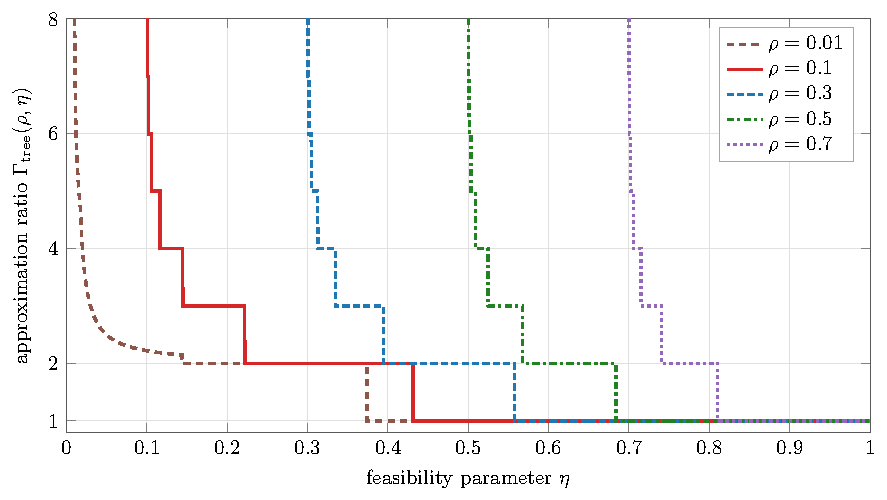
\includegraphics[width=0.92\textwidth]{figures/generated/tree_approximation_ratio_2d_plot.pdf}
  \caption{The combined approximation ratio from Corollary~\ref{cor:tree-best-bicriteria} as a function of $\eta$ for representative values of $\rho$. Values above $8$ are capped at $8$.}
  \label{fig:tree-approximation-ratio}
\end{figure}


\begin{figure}[!tbp]
  \centering
  % Rendered on demand from tree_approximation_ratio_3d_plot.tex.
  % Keeping the dense PGFPlots surface as a PDF avoids rebuilding it with
  % every manuscript compilation.
  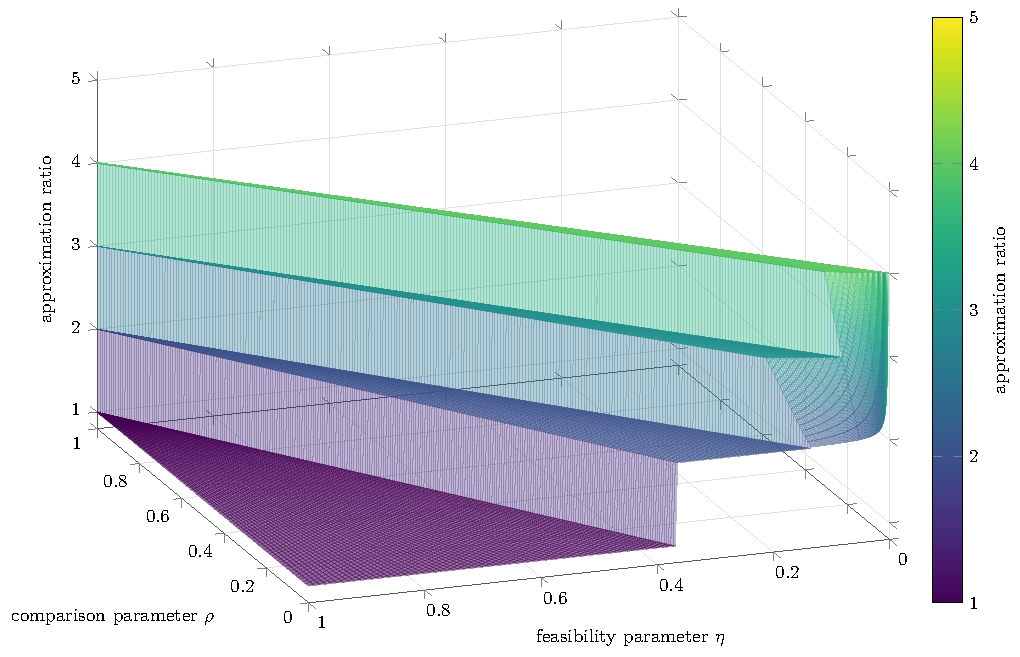
\includegraphics[width=0.94\textwidth]{figures/generated/tree_approximation_ratio_3d_plot.pdf}
  \caption{Combined tree approximation guarantee $\Gamma_{\mathrm{tree}}(\rho,\eta)$ from Corollary~\ref{cor:tree-best-bicriteria}, over $0<\rho<\eta<1$ (shown for $0.005\leq\rho\leq0.995$). Below the threshold, the height is the minimum of the anchored-LP, recursive, and hybrid bounds; above it, the direct dynamic program gives ratio $1$. Heights are capped at $12$. The plateaus reflect floor-log terms in the recursive and hybrid bounds.}
  \label{fig:tree-approximation-ratio-3d}
\end{figure}


\subsection{Consequences for hierarchical clustering on trees}

Combining Theorem~\ref{thm:tree-degree-config-direct} with Theorem~\ref{thm:hc-gpd-transfer} improves the tree guarantee for \textsc{Hierarchical Clustering with Demands}.

\begin{corollary}\label{cor:tree-hc-improved}
    For every rational $\varepsilon>0$, there is a polynomial-time $(8+\varepsilon)$-approximation algorithm for \textsc{Hierarchical Clustering with Demands} on supply trees.
\end{corollary}
\begin{proof}
    Set $\rho=1/2$ and choose $
        \eta=\frac{6+\varepsilon}{8+\varepsilon}.$
    Then $\eta>3/4=(1+\rho)/2$, so Theorem~\ref{thm:tree-degree-config-direct} gives $\gamma(\eta)=1$. The approximation guarantee from Theorem~\ref{thm:hc-gpd-transfer} is $
        \frac{2}{1-\eta}=8+\varepsilon.$
    Moreover, $2\cdot\eta-1-\rho=\varepsilon/(16+2\varepsilon)$, so the running time is polynomial in the input size and $1/\varepsilon$.
\end{proof}
